\documentclass[14pt]{beamer}
\usepackage{./Estilos/BeamerUVM}
\usepackage{./Estilos/ColoresLatex}
\input{Preambulos/preambulo_Beamer_Madrid_default}
% \usefonttheme{serif}
\usepackage[clock]{ifsym}

\sisetup{per-mode=symbol}
\resetcounteronoverlays{saveenumi}

\title{\Large{Descomposición de vectores} \\ \normalsize{Física 1}}
\date{26 de junio de 2023}

\begin{document}
\maketitle

\section*{Contenido}
\frame{\frametitle{Contenido} \tableofcontents[currentsection, hideallsubsections]}

\section{Avisos importantes}
\frame{\tableofcontents[currentsection, hideothersubsections]}
\subsection{En las clases}

\begin{frame}
\frametitle{Regreso a las clases presenciales}
Se debe de mantener en todo momento dentro del Campus San Rafael, un orden, disciplina y respeto.
\\
\bigskip
\pause
Hay que mantenerse atentos a la clase, sin distracciones o generando ruido.
\end{frame}
\begin{frame}
\frametitle{Pase de asistencia}
Como norma dentro de la clase, se llevará a cabo el Pase de Asistencia a los 6 minutos de iniciada la clase.
\\
\bigskip
\pause
En caso de ingresar luego de haber nombrado a la alumna/alumno, no se corregirá la inasistencia, a menos que se tenga un justificante por parte de la Coordinación Académica.
\end{frame}
\begin{frame}
\frametitle{Faltas en el período}
Como medida adicional, previo a la evaluación del segundo y tercer examen parcial, se presentará a cada alumno el total de inasistencias.
\end{frame}
\begin{frame}
\frametitle{Seguimiento de actividades}
De manera semanal, el Profesor enviará a cada alumna/alumno la relación de ejercicios de Evaluación Continua y de Prácticas que se hayan dejado en la semana anterior.
\\
\bigskip
\pause
El alumno también llevará su propio registro de actividades, esto nos facilitará el proceso de realizar las calificaciones correspondientes.
\end{frame}
\begin{frame}
\frametitle{Actividades en tiempo y forma}
El envío de actividades de Evaluación Continua y de Laboratorio, se seguirá realizando mediante Teams, con fecha y hora establecida de entrega.
\\
\bigskip
\pause
En caso de que se tenga un problema para enviar su documento, deberá de tomar evidencia del problema, \textocolor{magenta}{solo con evidencia se recibirá la actividad}.
\end{frame}
\begin{frame}
\frametitle{Actividades en tiempo y forma}
Cada actividad de trabajo formará parte de la segunda y tercera evaluación parcial.
\\
\bigskip
\pause
No habrá trabajos adicionales a modo de \enquote{compensar} las actividades no entregadas.
\end{frame}
\begin{frame}
\frametitle{Entrega de actividades}
Todo trabajo deberá ser enviado mediante Teams.
\\
\bigskip
\pause
Si el Profesor requiere que se envíe de nuevo un documento, él mismo solicitará mediante mensaje directo a la alumna/alumno. \pause Todo archivo que se reciba sin ser solicitado, no se atenderá, como tampoco será considerado como evidencia de entrega.
\end{frame}

\section{Descomposición de vectores}
\frame{\tableofcontents[currentsection, hideothersubsections]}
\subsection{Base geométrica}

\begin{frame}
\frametitle{Base geométrica}
\begin{figure}
    \centering
    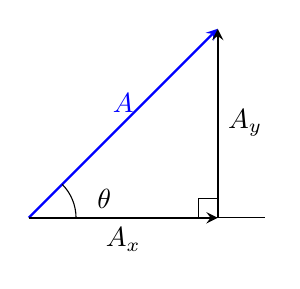
\begin{tikzpicture}[scale=1.2]
        \draw [-stealth, thick, color=blue] (0, 0) -- (2, 2) node [above, midway] {$\va{A}$};
        \draw (0.5, 0) arc(0:45:0.5);
        \node at (0.8, 0.2) {$\theta$};
        \draw (0, 0) -- (2.5, 0);
        \draw [-stealth, thick] (2, 0) -- (2, 2) node [right, midway] {$A_{y}$};
        \draw [-stealth, thick] (0, 0) -- (2, 0) node [below, midway] {$A_{x}$};
        \draw (1.8, 0) -- (1.8, 0.2) -- (2, 0.2);
    \end{tikzpicture}
\end{figure}
Las componentes del vector son:
\begin{eqnarray*}
\begin{aligned}
A_{x} &= \cos \theta \, \abs{A} \\[0.5em] \pause
A_{y} &= \sin \theta \, \abs{A}
\end{aligned}
\end{eqnarray*}
\end{frame}
\begin{frame}
\frametitle{Base geométrica}
\begin{figure}
    \centering
    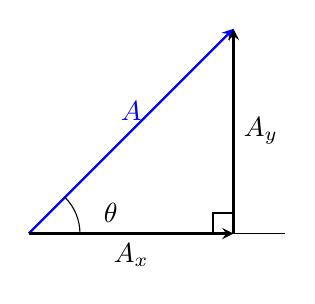
\begin{tikzpicture}[scale=1.3]
        \draw [-stealth, thick, color=blue] (0, 0) -- (2, 2) node [above, midway] {$\va{A}$};
        \draw (0.5, 0) arc(0:45:0.5);
        \node at (0.8, 0.2) {$\theta$};
        \draw (0, 0) -- (2.5, 0);
        \draw [-stealth, thick] (2, 0) -- (2, 2) node [right, midway] {$A_{y}$};
        \draw [-stealth, thick] (0, 0) -- (2, 0) node [below, midway] {$A_{x}$};
        \draw (1.8, 0) -- (1.8, 0.2) -- (2, 0.2);
    \end{tikzpicture}
\end{figure}
La magnitud del vector $\va{A}$ es:
\pause
\begin{align*}
\abs{\va{A}} = \sqrt{(A_{x})^{2} + (A_{y})^{2}}
\end{align*}
\end{frame}
\begin{frame}
\frametitle{Base geométrica}
\begin{figure}
    \centering
    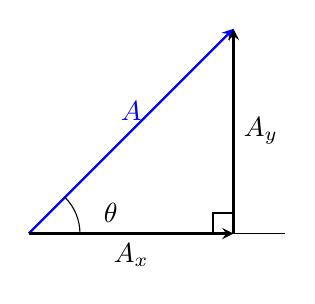
\begin{tikzpicture}[scale=1.3]
        \draw [-stealth, thick, color=blue] (0, 0) -- (2, 2) node [above, midway] {$\va{A}$};
        \draw (0.5, 0) arc(0:45:0.5);
        \node at (0.8, 0.2) {$\theta$};
        \draw (0, 0) -- (2.5, 0);
        \draw [-stealth, thick] (2, 0) -- (2, 2) node [right, midway] {$A_{y}$};
        \draw [-stealth, thick] (0, 0) -- (2, 0) node [below, midway] {$A_{x}$};
        \draw (1.8, 0) -- (1.8, 0.2) -- (2, 0.2);
    \end{tikzpicture}
\end{figure}
El valor del ángulo $\theta$ es:
\pause
\begin{align*}
\theta = \tan^{-1} \left( \dfrac{A_y}{A_{x}} \right)
\end{align*}
\end{frame}
\begin{frame}
\frametitle{Ejercicio}
Calcula las componentes del siguiente vector:
\pause
\begin{figure}
    \centering
    \includegraphics[scale=1.2]{Imagenes/Componentes_Vector_04.eps}
\end{figure}
\end{frame}
\begin{frame}
\frametitle{Resolviendo el Ejercicio}
Conocemos la magnitud del vector (\SI{5}{\newton}) y la dirección (el ángulo $\theta = \ang{30}$), por lo que hay que ocupar las expresiones:
\pause
\begin{eqnarray*}
\begin{aligned}
F_{x} &= \cos \theta \, \abs{A} \\[0.5em] \pause
F_{y} &= \sin \theta \, \abs{A}    
\end{aligned}
\end{eqnarray*}
\end{frame}
\begin{frame}
\frametitle{La componente en la dirección x}
Para calcular la componente del vector en la dirección $x$, sustituimos los valores 
\pause
\begin{eqnarray*}
\begin{aligned}
F_{x} &= \cos \theta \, \abs{A} =  \\[0.5em] \pause
F_{x} &= \cos (\ang{30}) \cdot (\SI{5}{\newton}) =  \\[0.5em] \pause
F_{x} &= (0.866) (\SI{5}{\newton}) =  \\[0.5em] \pause
F_{x} &= \SI{4.33}{\newton}
\end{aligned}
\end{eqnarray*}
\end{frame}    
\begin{frame}
\frametitle{La componente en la dirección y}
Para calcular la componente del vector en la dirección $y$, sustituimos los valores 
\pause
\begin{eqnarray*}
\begin{aligned}
F_{y} &= \sin \theta \, \abs{A} =  \\[0.5em] \pause
F_{y} &= \sin (\ang{30}) \cdot (\SI{5}{\newton}) =  \\[0.5em] \pause
F_{y} &= (0.5) (\SI{5}{\newton}) =  \\[0.5em] \pause
F_{y} &= \SI{2.5}{\newton}
\end{aligned}
\end{eqnarray*}
\end{frame}
\begin{frame}
\frametitle{Solución al ejercicio}
\begin{figure}
    \centering
    \includegraphics[scale=1.2]{Imagenes/Componentes_Vector_04.eps}
\end{figure}
\begin{tikzpicture}[overlay]
    \node at (2, 3) {$F_{x} = \SI{4.33}{\newton}$};
    \node at (2, 2) {$F_{y} = \SI{2.5}{\newton}$};
\end{tikzpicture}
\end{frame}
\begin{frame}
\frametitle{Ejercicio para la clase}
Calcula las componentes del vector:
\begin{figure}
    \centering
    \includegraphics[scale=1.3]{Imagenes/Componentes_Vector_05.eps}
\end{figure}
\end{frame}

\subsection{Vectores en otros cuadrantes}

\begin{frame}
\frametitle{Considera el siguiente vector}
\begin{figure}
    \centering
    \includegraphics[scale=1.5]{Imagenes/Componentes_Vector_06.eps}
\end{figure}
\end{frame}
\begin{frame}
\frametitle{Evaluando las funciones trigonométricas}
Podríamos calcular las funciones trigonométricas seno y coseno del ángulo de 150 grados.
\pause
\begin{eqnarray*}
\begin{aligned}
\cos \ang{150} &= -0.866 \\[0.5em] \pause
\sin \ang{150} &= 0.5
\end{aligned}
\end{eqnarray*}
\end{frame}
\begin{frame}
\frametitle{Simplificando las cuentas}
Recordando del curso de Matemáticas, aprovechamos mejor el ángulo suplementario, es decir, \pause el ángulo con el que se completan los 180 grados.
\end{frame}
\begin{frame}
\frametitle{Ángulo suplementario}
\begin{figure}
    \centering
    \includegraphics[scale=1.5]{Imagenes/Componentes_Vector_07.eps}
\end{figure}
\end{frame}
\begin{frame}
\frametitle{Detalle importante}
Veamos que al calcular las funciones seno y coseno del ángulo suplementario, en el ejemplo $\varphi = \ang{30}$, obtenemos los valores:
\pause
\begin{align*}
\cos \ang{30} &= 0.866 \\[0.5em]
\sin \ang{30} &= 0.5
\end{align*}
\end{frame}
\begin{frame}
\frametitle{Detalle importante}
Para la función coseno, el valor para el ángulo $\varphi = \ang{30}$, corresponde en magnitud que el valor del coseno de $\theta = \ang{150}$, pero NO le asocia es signo negativo.
\end{frame}
\begin{frame}
\frametitle{Detalle importante}
Por lo que tendremos que anotar el signo negativo en la operación que corresponde para la componente en el eje $x$ de un vector.
\\
\bigskip
\pause
La componente en el eje $x$, tiene su sentido en el eje $x$ negativo.
\end{frame}

\begin{frame}
\frametitle{Usando el ángulo suplementario}
Una vez identificado el ángulo suplementario, procedemos a calcular las componentes del vector.
\pause
\begin{eqnarray*}
\begin{aligned}
d_{x} &= - \cos \theta \, \abs{d} =  \\[0.5em] \pause
&= - \cos (\ang{30}) \cdot (\SI[per-mode=symbol]{10}{\meter\per\second}) =  \\[0.5em] \pause
&= - (0.866) (\SI[per-mode=symbol]{10}{\meter\per\second}) =  \\[0.5em] \pause
&= - \SI[per-mode=symbol]{8.66}{\meter\per\second}
\end{aligned}
\end{eqnarray*}
\end{frame}
\begin{frame}
\frametitle{Usando el ángulo suplementario}
Para la componente en el eje $y$ del vector $\va{d}$:
\pause
\begin{eqnarray*}
\begin{aligned}
d_{y} &= \sin \theta \, \abs{d} =  \\[0.5em] \pause
&= \sin (\ang{30}) \cdot (\SI[per-mode=symbol]{10}{\meter\per\second}) =  \\[0.5em] \pause
&= (0.5) (\SI[per-mode=symbol]{10}{\meter\per\second}) =  \\[0.5em] \pause
&= \SI[per-mode=symbol]{5}{\meter\per\second}
\end{aligned}
\end{eqnarray*}
\end{frame}
\begin{frame}
\frametitle{Revisión importante}
Nota que la componente del vector en la dirección $x$, tiene un valor negativo.
\\
\bigskip
Esto nos indica el sentido del vector, \textocolor{cobalt}{la magnitud siempre es un valor positivo}.
\end{frame}
\begin{frame}
\frametitle{¿Qué pasa con los cuadrantes III y IV?}
Al descomponer un vector, debes de verificar en qué cuadrante se encuentra, \pause ya que de esa manera, te dará una guía para determinar el signo de las componentes, como se vio en el caso de un vector en el cuadrante II.
\end{frame}
\begin{frame}
\frametitle{El cuadrante III}
Considera que un vector en el cuadrante III, tendrá siempre la componente en el eje $x$ con un signo negativo, \pause y la componente en el eje $y$, también con signo negativo, como se muestra a continuación.
\end{frame}
\begin{frame}
\frametitle{El cuadrante III}
\begin{figure}
    \centering
    \includegraphics[scale=1.25]{Imagenes/Componentes_Vector_08.eps}
\end{figure}
\end{frame}
\begin{frame}
\frametitle{¿Con qué ángulo se trabajaría en el cuadrante III?}
Cuando tengamos un vector en el cuadrante III, podemos ocupar un ángulo complementario para simplificar las operaciones.
\end{frame}
\begin{frame}
\frametitle{El ángulo de trabajo}
\begin{figure}
    \centering
    \includegraphics[scale=1.3]{Imagenes/Componentes_Vector_08a.eps}
\end{figure}
\end{frame}
\begin{frame}
\frametitle{Las componentes del vector}
Las componentes del vector $\va{C}$ en el cuadrante III, son entonces:
\begin{align*}
C_{x} & = - \cos \alpha \cdot \abs{\va{C}} \\[0.5em]
C_{y} & = - \sin \alpha \cdot \abs{\va{C}}
\end{align*}
\end{frame}
\begin{frame}
\frametitle{El cuadrante IV}
Mientras que un vector en el cuadrante IV, tendrá siempre la componente en el eje $x$ con un signo positivo, \pause y la componente en el eje $y$, con signo negativo.
\end{frame}
\begin{frame}
\frametitle{El cuadrante IV}
\begin{figure}
    \centering
    \includegraphics[scale=1.3]{Imagenes/Componentes_Vector_09.eps}
\end{figure}
\end{frame}
\begin{frame}
\frametitle{Usando el ángulo complementario}
Ahora consideramos el ángulo complementario en el cuadrante IV, como se muestra en la siguiente figura:
\end{frame}
\begin{frame}
\frametitle{Usando el ángulo complementario}
\begin{figure}
    \centering
    \includegraphics[scale=1.3]{Imagenes/Componentes_Vector_09a.eps}
\end{figure}
\end{frame}
\begin{frame}
\frametitle{Las componentes del vector}
Las componentes del vector $\va{M}$ en el cuadrante IV, son entonces:
\begin{align*}
M_{x} & = \cos \psi \cdot \abs{\va{M}} \\[0.5em]
M_{y} & = - \sin \psi \cdot \abs{\va{M}}
\end{align*}
\end{frame}
    
\section{Método analítico}
\frame{\tableofcontents[currentsection, hideothersubsections]}
\subsection{Obteniendo la resultante}

\begin{frame}
\frametitle{Planteamiento}
Consideremos un conjunto de vectores:
\pause
\begin{align*}
\va{F}_{1}, \va{F}_{2}, \va{F}_{3}, \va{F}_{4}
\end{align*}
que están interactuando sobre un objeto.
\end{frame}
\begin{frame}
\frametitle{El vector resultante}
Podemos considerar que sobre ese objeto actúa un solo vector, \pause que es la suma vectorial de esos vectores individuales: \pause \textocolor{red}{el vector resultante}.
\pause
\begin{align*}
\va{R} = \va{F}_{1} + \va{F}_{2} + \va{F}_{3} + \va{F}_{4} 
\end{align*}
\end{frame}
\begin{frame}
\frametitle{El método analítico}
El método analítico consiste en obtener el vector resultante, a partir de las componentes en el eje $x$ y en el eje $y$.
\\
\bigskip
\pause
Sumando las componentes en cada eje, de cada vector.
\end{frame}
\begin{frame}
\frametitle{Las componentes del vector resultante}
Es decir:
\pause
\begin{eqnarray*}
\begin{aligned}
R_{x} &= F_{1x} + F_{2x} + F_{3x} + F_{4x} = \pause \nsum_{i=1}^{4} F_{ix} \\[0.5em] \pause 
R_{y} &= F_{1y} + F_{2y} + F_{3y} + F_{4y} = \pause \nsum_{i=1}^{4} F_{iy}
\end{aligned}
\end{eqnarray*}
\end{frame}
\begin{frame}
\frametitle{La magnitud del vector resultante}
Una vez obtenidas las componentes del vector resultante, \pause es posible calcular la magnitud del mismo:
\pause
\begin{align*}
\abs{\va{R}} = \sqrt{(R_{x})^{2} + (R_{y})^{2}}
\end{align*}
\end{frame}
\begin{frame}
\frametitle{La dirección del vector resultante}
La última parte que nos falta, es determinar la dirección del vector, mediante el ángulo que forma con respecto al eje $x$ positivo:
\pause
\begin{eqnarray*}
\begin{aligned}
\tan \theta &= \dfrac{R_{y}}{R_{x}} \\[0.3em] \pause
\arctan(\tan \theta) &= \arctan(\dfrac{R_{y}}{R_{x}}) \\[0.5em] \pause
\theta &= \arctan(\dfrac{R_{y}}{R_{x}}) = \pause \tan^{-1} \left( \dfrac{R_{y}}{R_{x}} \right)
\end{aligned}
\end{eqnarray*}
\end{frame}

\section{Ejercicios a Detalle}
\frame{\tableofcontents[currentsection, hideothersubsections]}
\subsection{Ejercicio 1}

\begin{frame}
\frametitle{Enunciado del Ejercicio 1}
Del siguiente sistema de vectores determina por el método analítico el valor de la resultante y el ángulo que forma con respecto al eje $x$ positivo.
\end{frame}
\begin{frame}[plain]
\begin{figure}
\centering
\begin{tikzpicture}[scale=0.8]
    \draw (-4, 0) -- (9, 0) node [above, pos=1] {$x$};
    \draw (0, -4) -- (0, 6) node [left, pos=1] {$y$};
    \draw [-stealth, line width=0.5mm, color=blue] (0, 0) -- (8, 0) node [below, midway] {$\va{F}_{1} = \SI{8}{\newton}$};
    \draw [-stealth, line width=0.5mm, color=burgundy] (0, 0) -- (4.59, 3.85) node [above, near end, rotate=40] {$\va{F}_{2} = \SI{6}{\newton}$};
    \draw [color=burgundy] (0.5, 0) arc(0:40:0.5);
    \node [color=burgundy] at (2, 0.4) {$\theta_{2} = \ang{40}$};
    \draw [-stealth, line width=0.5mm, color=cerise] (0, 0) -- (-2.59, -1.5) node [below, near end, rotate=30] {$\va{F}_{3} = \SI{3}{\newton}$};
    \draw [color=cerise] (-0.5, 0) arc(180:210:0.5);
    \node [color=cerise] at (-2,- 0.3) {$\theta_{3} = \ang{30}$};
    \draw [-stealth, line width=0.5mm, color=byzantine] (0, 0) -- (0, 5) node [left, near end] {$\va{F}_{4} = \SI{5}{\newton}$};
\end{tikzpicture}
\end{figure}
\end{frame}
\begin{frame}
\frametitle{Recomendación para la solución}
Es conveniente enlistar los vectores involucrados de tal manera que tengamos identificado: el cuadrante en el que se encuentra cada vector, así como su magnitud y el ángulo.
\end{frame}
\begin{frame}
\frametitle{Recomendación para la solución}
Recordemos que todo vector debe de tener un ángulo asociado, veremos en particular que en el ejercicio hay dos vectores que coinciden con los ejes del sistema cartesiano.
\end{frame}
\begin{frame}
\frametitle{Lista de vectores}
\begin{table}
\centering
\begin{tabular}{c | c | c | c }
Vector & Cuadrante & Magnitud (en $\unit{\newton}$) & Ángulo \\ \hline
$\va{F}_{1}$ & I / IV & $8$ & $\theta_{1} = \ang{0}$ \\ \hline
$\va{F}_{2}$ & I & $6$ & $\theta_{2} = \ang{40}$ \\ \hline
$\va{F}_{3}$ & III & $3$ & $\theta_{3} = \ang{30}$ \\ \hline
$\va{F}_{4}$ & I / II & $5$ & $\theta_{4} = \ang{90}$ \\ \hline
\end{tabular}
\end{table}
\end{frame}
\begin{frame}
\frametitle{Calculando las componentes}
Una vez que tenemos la lista de vectores, iniciamos el cálculo de las componentes en las direcciones $x$ e $y$ de cada uno de ellos.
\\
\bigskip
\pause
Siendo recomendable también hacer una tabla con las componentes.
\end{frame}
\begin{frame}
\frametitle{Tabla con las componentes}
\begin{table}
\centering
\begin{tabular}{c | l | l | c}
Componente & Expresión & Sustitución & Valor \\ \hline
$F_{1x}$ & $\cos \theta_{1} \cdot F_{1}$ & $\cos \ang{0} \cdot \SI{8}{\newton}$ & $\SI{8}{\newton}$ \\ \hline
$F_{1y}$ & $\sin \theta_{1} \cdot F_{1}$ & $\sin \ang{0} \cdot \SI{8}{\newton}$ & $\SI{0}{\newton}$ \\ \hline
$F_{2x}$ & $\cos \theta_{2} \cdot F_{2}$ & $\cos \ang{40} \cdot \SI{6}{\newton}$ & $\SI{4.59}{\newton}$ \\ \hline
$F_{2y}$ & $\sin \theta_{2} \cdot F_{2}$ & $\sin \ang{40} \cdot \SI{6}{\newton}$ & $\SI{3.85}{\newton}$ \\ \hline
\end{tabular}
\end{table}
\end{frame}
\begin{frame}
\frametitle{Tabla con las componentes}
\begin{table}
\centering
\begin{tabular}{c | l | l | c}
Componente & Expresión & Sustitución & Valor \\ \hline
$F_{3x}$ & $-\cos \theta_{3} \cdot F_{3}$ & $-\cos \ang{30} \cdot \SI{3}{\newton}$ & $-\SI{2.59}{\newton}$ \\ \hline
$F_{3y}$ & $-\sin \theta_{3} \cdot F_{3}$ & $-\sin \ang{30} \cdot \SI{3}{\newton}$ & $-\SI{1.5}{\newton}$ \\ \hline
$F_{4x}$ & $\cos \theta_{4} \cdot F_{4}$ & $\cos \ang{90} \cdot \SI{5}{\newton}$ & $\SI{0}{\newton}$ \\ \hline
$F_{4y}$ & $\sin \theta_{4} \cdot F_{4}$ & $\sin \ang{90} \cdot \SI{5}{\newton}$ & $\SI{5}{\newton}$ \\ \hline
\end{tabular}
\end{table}
\end{frame}
\begin{frame}
\frametitle{Componentes del vector resultante}
Ahora ya podemos calcular las componentes del vector resultante, \pause recordemos que la componente en la dirección $x$ es:
\pause
\begin{eqnarray*}
\begin{aligned}
R_{x} &= \nsum_{i=1}^{4} F_{ix} = \pause F_{1x} + F_{2x} + F_{3x} + F_{4x} = \\[0.5em] \pause
&= \SI{8}{\newton} {+} \SI{4.59}{\newton} {+} (-\SI{2.59}{\newton}) {+} \SI{0}{\newton} = \\[0.5em] \pause
&= \SI{10}{\newton}
\end{aligned}
\end{eqnarray*}
\end{frame}
\begin{frame}
\frametitle{Componentes del vector resultante}
Para la componente en la dirección $y$ del vector resultante $R_{y}$:
\pause
\begin{eqnarray*}
\begin{aligned}
R_{y} &= \nsum_{i=1}^{4} F_{iy} = \pause F_{1y} + F_{2y} + F_{3y} + F_{4y} = \\[0.5em] \pause
&= \SI{0}{\newton} {+} \SI{3.85}{\newton} {+} (-\SI{1.5}{\newton}) {+} \SI{5}{\newton} = \\[0.5em] \pause
&= \SI{7.35}{\newton}
\end{aligned}
\end{eqnarray*}
\end{frame}
\begin{frame}
\frametitle{Magnitud del vector resultante}
Una vez obtenidas las componentes en $x$ e $y$, calculamos la magnitud del vector resultante:
\pause
\begin{eqnarray*}
\begin{aligned}
\abs{\va{R}} &= \sqrt{(R_{x})^{2} + (R_{y})^{2}} = \\[0.5em] \pause
\abs{\va{R}} &= \sqrt{(\SI{10}{\newton})^{2} + (\SI{7.35}{\newton})^{2}} = \\[0.5em] \pause
\abs{\va{R}} &= \sqrt{\SI{100}{\square\newton} + \SI{54.02}{\square\newton}} = \pause \sqrt{\SI{154.02}{\square\newton}} = \\[0.5em] \pause
\abs{\va{R}} &= \SI{12.41}{\newton}
\end{aligned}
\end{eqnarray*}
\end{frame}
\begin{frame}
\frametitle{El ángulo del vector resultante}
Tenemos que $R_{x} > 0$ y $R_{y} > 0$, \pause por lo que el vector resultante está en el cuadrante I, \pause con esos valores podemos calcular el valor del ángulo del vector resultante con respecto al eje $x$ positivo:
\end{frame}
\begin{frame}
\frametitle{El ángulo del vector resultante}
El ángulo $\theta_{R}$ resulta ser:
\pause
\begin{eqnarray*}
\begin{aligned}
\tan \theta_{R} &= \dfrac{R_{y}}{R_{x}} = \pause
    \dfrac{\SI{7.35}{\newton}}{\SI{10}{\newton}} = \pause  0.735 \\[0.5em] \pause
\arctan(\tan \theta_{R}) &= \arctan(0.735) \\[0.5em] \pause
\theta_{R} &= \ang{36.31}
\end{aligned}
\end{eqnarray*}
\end{frame}
\begin{frame}[plain]
\begin{figure}
\frametitle{El vector resultante: magnitud y dirección}
\centering
\begin{tikzpicture}[scale=0.5]
    \draw (-4, 0) -- (9, 0) node [above, pos=1] {$x$};
    \draw (0, -4) -- (0, 6) node [left, pos=1] {$y$};
    \draw [-stealth, thick, color=blue] (0, 0) -- (8, 0) node [below, midway] {\small{$\va{F}_{1}$}};

    \draw [-stealth, thick, color=burgundy] (0, 0) -- (4.59, 3.85) node [above, near end, rotate=40] {\small{$\va{F}_{2}$}};
    \draw [color=burgundy] (0.5, 0) arc(0:40:0.5);
    \node [color=burgundy] at (1.6, 0.4) {\small{$\theta_{2}$}};

    \draw [-stealth, thick, color=cerise] (0, 0) -- (-2.59, -1.5) node [below, near end, rotate=30] {\small{$\va{F}_{3}$}};
    \draw [color=cerise] (-0.5, 0) arc(180:210:0.5);
    \node [color=cerise] at (-1.8,- 0.4) {\small{$\theta_{3}$}};

    \draw [-stealth, thick, color=byzantine] (0, 0) -- (0, 5) node [left, near end] {\small{$\va{F}_{4}$}};
    
    \draw [-stealth, line width=0.5mm, color=cadmiumred] (0, 0) -- (9.69, 7.35) node [above, near end, rotate=37] {\small{$\va{R} = \SI{12.41}{\newton}$}};
    \draw [thick, color=cadmiumred] (3, 0) arc(0:37:3);
    \node [color=cadmiumred] at (5.2, 0.8) {\small{$\theta_{R} = \ang{36.31}$}};
\end{tikzpicture}
\end{figure}
\end{frame}

\subsection{Ejercicios a cuenta}

\begin{frame}
\frametitle{Enunciado del ejercicio a cuenta 1}
Realiza la suma de los siguientes tres vectores, determinando el vector resultante y el ángulo que forma la resultante con respecto al eje $x$ positivo.
\end{frame}
\begin{frame}
\frametitle{Diagrama para el Ejercicio 1}
\begin{figure}
\centering
\begin{tikzpicture}
    \draw (-6, 0) -- (2, 0);
    \draw (0, -2) -- (0, 1.5);
    \draw [-stealth, line width=0.5mm, color=ao] (0, 0) -- (1.69, 0.61) node [above, pos=1.2] {\small{$T_{1} = \SI{18}{\newton}$}};
    \draw [color=ao] (0.5, 0) arc(0:20:0.4);
    \node at (2, 0.2) [color=ao] {\small{$\theta_{1} = \ang{20}$}};

    \draw [-stealth, line width=0.5mm, color=darkmagenta] (0, 0) -- (-5.6, 0) node [above, near end] {\small{$T_{3} = \SI{58}{\newton}$}};
    \draw [color=darkmagenta] (0.4, 0) arc(0:180:0.5);
    \node at (-1.5, 0.4) [color=darkmagenta] {\small{$\theta_{3} = \ang{180}$}};
    
    \draw [-stealth, line width=0.5mm, color=officegreen] (0, 0) -- (0.306, -0.629) node [above, xshift=0.5cm, yshift=-0.7cm] {\small{$T_{2} = \SI{7}{\newton}$}};
    \draw [color=officegreen] (0.3, 0) arc(360:296:0.3);
    \node at (1.3, -0.4) [color=officegreen] {\small{$\theta_{2} = \ang{64}$}};
\end{tikzpicture}
\end{figure}
\end{frame}
\begin{frame}
\frametitle{Ejercicio 2}
Realiza la suma de los vectores que se muestran en la siguiente figura, calculando la magnitud del vector resultante, así como la dirección del mismo.
\end{frame}
\begin{frame}
\begin{figure}
    \centering
    \begin{tikzpicture}[scale=0.5]
    \draw (-4, 0) -- (5, 0);
    \draw (0, -9) -- (0, 5);
    \draw [-stealth, line width=0.5mm, color=carmine] (0, 0) -- (4.17, 4.17) node [above, pos=1] {\small{$F_{1} = \SI{59}{\newton}$}};
    \draw [color=carmine] (0.5, 0) arc(0:45:0.5);
    \node at (2.5, 0.3) [color=carmine] {\small{$\theta_{1} = \ang{45}$}};

    \draw [-stealth, line width=0.5mm, color=electricindigo] (0, 0) -- (1.97, -1.18) node [above, xshift=0.8cm, yshift=-0.7cm] {\small{$F_{2} = \SI{23}{\newton}$}};
    \draw [color=electricindigo] (0.5, 0) arc(360:329:0.5);
    \node at (2.8, -0.5) [color=electricindigo] {\small{$\theta_{2} = \ang{31}$}};
    
    \draw [-stealth, line width=0.5mm, color=officegreen] (0, 0) -- (-0.919, -8.75) node [left, midway] {\small{$F_{3} = \SI{88}{\newton}$}};
    \draw [color=officegreen] (-0.5, 0) arc(180:264:0.5);
    \node at (-2, -0.5) [color=officegreen] {\small{$\theta_{3} = \ang{84}$}};

    \draw [-stealth, line width=0.5mm, color=persimmon] (0, 0) -- (-0.745, 1.52) node [above, xshift=-1cm, yshift=-0.2cm] {\small{$F_{4} = \SI{17}{\newton}$}};
    \draw [thick, color=persimmon] (-0.5, 0) arc(180:116:0.5);
    \node at (-2, 0.5) [color=persimmon] {\small{$\theta_{4} = \ang{64}$}};
\end{tikzpicture}
\end{figure}
\end{frame}
\begin{frame}
\frametitle{Puntaje de los ejercicios}
Cada ejercicio aporta un punto en Evaluación Continua.
\\
\bigskip
\pause
La solución de enviará por Teams, el plazo vence el domingo 2 de julio a las 8 pm.
\end{frame}
\begin{frame}
\frametitle{Cumplimiento en tiempo y forma}
No se recibirán trabajos extemporáneos, a menos que se tenga la evidencia de problemas durante el envío, y que hayan sido notificados al momento, tanto en la Coordinación Académica como al Profesor.
\end{frame}
\end{document}